From \probref{chapters/11/10/2/15},
\begin{align}
	\vec{n} = \myvec{-1\\2} \implies m = \frac{1}{2}
\end{align}
Also, from the given equation of the line and the given point, 
\begin{align}
	c = \myvec{-m & 1}\myvec{-1\\2} = 
\frac{5}{2}  
\end{align}
\iffalse
 See \figref{fig:pic}.
\begin{figure}[H]
 \centering
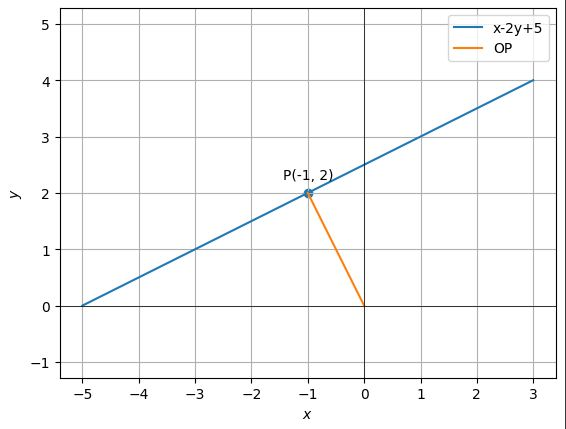
\includegraphics[width=0.75\columnwidth]{chapters/11/10/3/15/figs/graph.jpg}
 \caption{Graph}
 \label{fig:pic}
\end{figure}
\fi
